% cpu/overheads.tex
% mainfile: ../perfbook.tex
% SPDX-License-Identifier: CC-BY-SA-3.0

\section{Overheads}
\label{sec:cpu:Overheads}
%
\epigraph{Don't design bridges in ignorance of materials, and don't design
	  low-level software in ignorance of the underlying hardware.}
	 {\emph{Unknown}}

This section presents actual overheads of the obstacles to performance
listed out in the previous section.
However, it is first necessary to get a rough view of hardware system
architecture, which is the subject of the next section.

\subsection{Hardware System Architecture}
\label{sec:cpu:Hardware System Architecture}

\begin{figure}[tb]
\centering
\resizebox{3in}{!}{\includegraphics{cpu/SystemArch}}
\caption{System Hardware Architecture}
\label{fig:cpu:System Hardware Architecture}
\end{figure}

Figure~\ref{fig:cpu:System Hardware Architecture}
shows a rough schematic of an eight-core computer system.
Each die has a pair of CPU cores, each with its cache, as well as an
interconnect allowing the pair of CPUs to communicate with each other.
The system interconnect allows the four dies to communicate with each
other and with main memory.

Data moves through this system in units of ``cache lines'', which
are power-of-two fixed-size aligned blocks of memory, usually ranging
from 32 to 256 bytes in size.
When a CPU loads a variable from memory to one of its registers, it must
first load the cacheline containing that variable into its cache.
Similarly, when a CPU stores a value from one of its registers into
memory, it must also load the cacheline containing that variable into
its cache, but must also ensure that no other CPU has a copy of that
cacheline.

For example, if CPU~0 were to write to a variable whose cacheline
resided in CPU~7's cache, the following over-simplified sequence of
events might ensue:

\begin{enumerate}
\item	CPU~0 checks its local cache, and does not find the cacheline.
	It therefore records the write in its store buffer.
\item	A request for this cacheline is forwarded to CPU~0's and 1's
	interconnect, which checks CPU~1's local cache, and does not
	find the cacheline.
\item	This request is forwarded to the system interconnect, which
	checks with the other three dies, learning that the cacheline
	is held by the die containing CPU~6 and 7.
\item	This request is forwarded to CPU~6's and 7's interconnect, which
	checks both CPUs' caches, finding the value in CPU~7's cache.
\item	CPU~7 forwards the cacheline to its interconnect, and also
	flushes the cacheline from its cache.
\item	CPU~6's and 7's interconnect forwards the cacheline to the
	system interconnect.
\item	The system interconnect forwards the cacheline to CPU~0's and 1's
	interconnect.
\item	CPU~0's and 1's interconnect forwards the cacheline to CPU~0's
	cache.
\item	CPU~0 can now complete the write, updating the relevant portions
	of the newly arrived cacheline from the value previously
	recorded in the store buffer.
\end{enumerate}

\QuickQuizSeries{%
\QuickQuizB{
	This is a \emph{simplified} sequence of events?
	How could it \emph{possibly} be any more complex?
}\QuickQuizAnswerB{
	This sequence ignored a number of possible complications,
	including:

	\begin{enumerate}
	\item	Other CPUs might be concurrently attempting to perform
		memory-reference operations involving this same cacheline.
	\item	The cacheline might have been replicated read-only in
		several CPUs' caches, in which case, it would need to
		be flushed from their caches.
	\item	CPU~7 might have been operating on the cache line when
		the request for it arrived, in which case CPU~7 might
		need to hold off the request until its own operation
		completed.
	\item	CPU~7 might have ejected the cacheline from its cache
		(for example, in order to make room for other data),
		so that by the time that the request arrived, the
		cacheline was on its way to memory.
	\item	A correctable error might have occurred in the cacheline,
		which would then need to be corrected at some point before
		the data was used.
	\end{enumerate}

	Production-quality cache-coherence mechanisms are extremely
	complicated due to these sorts of
	considerations~\cite{Hennessy95a,DavidECuller1999,MiloMKMartin2012scale,DanielJSorin2011MemModel}.
%
}\QuickQuizEndB
%
\QuickQuizE{
	Why is it necessary to flush the cacheline from CPU~7's cache?
}\QuickQuizAnswerE{
	If the cacheline was not flushed from CPU~7's cache, then
	CPUs~0 and 7 might have different values for the same set
	of variables in the cacheline.
	This sort of incoherence greatly complicates parallel software,
	which is why so wise hardware architects avoid it.
}\QuickQuizEndE
}

This simplified sequence is just the beginning of a discipline called
\emph{cache-coherency protocols}~\cite{Hennessy95a,DavidECuller1999,MiloMKMartin2012scale,DanielJSorin2011MemModel},
which is discussed in more detail in
Appendix~\ref{chp:app:whymb:Why Memory Barriers?}.
As can be seen in the sequence of events triggered by a CAS operation,
a single instruction can cause considerable protocol traffic, which
can significantly degrade your parallel program's performance.

Fortunately, if a given variable is being frequently read during a time
interval during which it is never updated, that variable can be replicated
across all CPUs' caches.
This replication permits all CPUs to enjoy extremely fast access to
this \emph{read-mostly} variable.
Chapter~\ref{chp:Deferred Processing} presents synchronization
mechanisms that take full advantage of this important hardware read-mostly
optimization.

\subsection{Costs of Operations}
\label{sec:cpu:Costs of Operations}

\begin{table*}
\rowcolors{1}{}{lightgray}
\renewcommand*{\arraystretch}{1.1}
\centering\small
\begin{tabular}
  {
    l
    S[table-format = 9.1]
    S[table-format = 9.1]
    r
  }
	\toprule
	Operation	   & \multicolumn{1}{r}{Cost (ns)}
				   & {\parbox[b]{.7in}{\raggedleft Ratio\\(cost/clock)}}
					    & CPUs \\
	\midrule
	Clock period		     &   0.5 &    1.0 &			  \\
	Same-CPU CAS		     &   7.0 &   14.6 & 0		  \\
	Same-CPU lock		     &  15.4 &   32.3 & 0		  \\
	In-core blind CAS	     &   7.2 &   15.2 & 224		  \\
	In-core CAS		     &  18.0 &   37.7 & 224		  \\
	Off-core blind CAS	     &  47.5 &   99.8 & 1--27,225--251	  \\
	Off-core CAS		     & 101.9 &  214.0 & 1--27,225--251	  \\
	Off-socket blind CAS	     & 148.8 &  312.5 & 28--111,252--335  \\
	Off-socket CAS		     & 442.9 &  930.1 & 28--111,252--335  \\
	Cross-interconnect blind CAS & 336.6 &  706.8 & 112--223,336--447 \\
	Cross-interconnect CAS	     & 944.8 & 1984.2 & 112--223,336--447 \\
	\midrule
	Off-System	&	      & 	    & \\
	Comms Fabric	&       5 000 &      10 500 & \\
	Global Comms	& 195 000 000 & 409 500 000 & \\
	\bottomrule
\end{tabular}
\caption{CPU 0 View of Synchronization Mechanisms on 8-Socket System With Intel Xeon Platinum 8176 CPUs @ 2.10\,GHz}
\label{tab:cpu:CPU 0 View of Synchronization Mechanisms on 8-Socket System With Intel Xeon Platinum 8176 CPUs at 2.10GHz}
\end{table*}

The overheads of some common operations important to parallel programs are
displayed in
Table~\ref{tab:cpu:CPU 0 View of Synchronization Mechanisms on 8-Socket System With Intel Xeon Platinum 8176 CPUs at 2.10GHz}.
This system's clock period rounds to 0.5\,ns.
Although it is not unusual for modern microprocessors to be able to
retire multiple instructions per clock period, the operations' costs are
nevertheless normalized to a clock period in the third column, labeled
``Ratio''.
The first thing to note about this table is the large values of many of
the ratios.

The same-CPU compare-and-swap (CAS) operation consumes about seven
nanoseconds, a duration more than ten times that of the clock period.
CAS is an atomic operation in which the hardware compares the contents
of the specified memory location to a specified ``old'' value, and if
they compare equal, stores a specified ``new'' value, in which case the
CAS operation succeeds.
If they compare unequal, the memory location keeps its (unexpected) value,
and the CAS operation fails.
The operation is atomic in that the hardware guarantees that the memory
location will not be changed between the compare and the store.
CAS functionality is provided by the \co{lock;cmpxchg} instruction on x86.

The ``same-CPU'' prefix means that the CPU now performing the CAS operation
on a given variable was also the last CPU to access this variable, so
that the corresponding cacheline is already held in that CPU's cache.
Similarly, the same-CPU lock operation (a ``round trip'' pair consisting
of a lock acquisition and release) consumes more than fifteen nanoseconds,
or more than thirty clock cycles.
The lock operation is more expensive than CAS because it requires two
atomic operations on the lock data structure, one for acquisition and
the other for release.

In-core operations involving interactions between the hardware threads
sharing a single core are about the same cost as same-CPU operations.
This should not be too surprising, given that these two hardware threads
also share the full cache hierarchy.

In the case of the blind CAS, the software specifies the old value
without looking at the memory location.
This approach is appropriate when attempting to acquire a lock.
If the unlocked state is represented by zero and the locked state
is represented by the value one, then a CAS operation on the lock
that specifies zero for the old value and one for the new value
will acquire the lock if it is not already held.
The key point is that there is only one access to the memory
location, namely the CAS operation itself.

In contrast, a normal CAS operation's old value is derived from
some earlier load.
For example, to implement an atomic increment, the current value of
that location is loaded and that value is incremented to produce the
new value.
Then in the CAS operation, the value actually loaded would be specified
as the old value and the incremented value as the new value.
If the value had not been changed between the load and the CAS, this
would increment the memory location.
However, if the value had in fact changed, then the old value would
not match, causing a miscompare that would result in the CAS operation
failing.
The key point is that there are now two accesses to the memory location,
the load and the CAS\@.

Thus, it is not surprising that in-core blind CAS consumes only about
seven nanoseconds, while in-core CAS consumes about 18 nanoseconds.
The non-blind case's extra load does not come for free.
That said, the overhead of these operations are similar to single-CPU
CAS and lock, respectively.

\QuickQuiz{
	\Cref{tab:cpu:CPU 0 View of Synchronization Mechanisms on 8-Socket System With Intel Xeon Platinum 8176 CPUs at 2.10GHz}
	shows CPU~0 sharing a core with CPU~224.
	Shouldn't that instead be CPU~1???
}\QuickQuizAnswer{
	It is easy to be sympathetic to this view, but the file
	\path{/sys/devices/system/cpu/cpu0/cache/index0/shared_cpu_list}
	really does contain the string \co{0,224}.
	Therefore, CPU~0's hyperthread twin really is CPU~224.
	Some people speculate that this numbering allows naive applications
	and schedulers to perform better, citing the fact that on many
	workloads the second hyperthread does not provide a huge
	amount of additional performance.
	This speculation assumes that naive applications and schedulers
	would utilize CPUs in numerical order, leaving aside the weaker
	hyperthread twin CPUs until all cores are in use.
}\QuickQuizEnd

A blind CAS involving CPUs in different cores but on the same socket
consumes almost fifty nanoseconds, or almost one hundred clock cycles.
The code used for this cache-miss measurement passes the cache line
back and forth between a pair of CPUs, so this cache miss is satisfied
not from memory, but rather from the other CPU's cache.
A non-blind CAS operation, which as noted earlier must look at the old
value of the variable as well as store a new value, consumes over one
hundred nanoseconds, or more than two hundred clock cycles.
Think about this a bit.
In the time required to do \emph{one} CAS operation, the CPU could have
executed more than \emph{two hundred} normal instructions.
This should demonstrate the limitations not only of fine-grained locking,
but of any other synchronization mechanism relying on fine-grained
global agreement.

If the pair of CPUs are on different sockets, the operations are considerably
more expensive.
A blind CAS operation consumes almost 150~nanoseconds, or more than
three hundred clock cycles.
A normal CAS operation consumes more than 400~nanoseconds, or almost
\emph{one thousand} clock cycles.

Worse yet, not all pairs of sockets are created equal.
This particular system appears to be constructed as a pair of four-socket
components, with additional latency penalties when the CPUs reside
in different components.
In this case, a blind CAS operation consumes more than three hundred
nanoseconds, or more than seven hundred clock cycles.
A CAS operation consumes almost a full microsecond, or almost two
thousand clock cycles.

\QuickQuiz{
	Surely the hardware designers could be persuaded to improve
	this situation!
	Why have they been content with such abysmal performance
	for these single-instruction operations?
}\QuickQuizAnswer{
	The hardware designers \emph{have} been working on this
	problem, and have consulted with no less a luminary than
	the late physicist Stephen Hawking.
	Hawking's observation was that the hardware designers have
	two basic problems~\cite{BryanGardiner2007}:

	\begin{enumerate}
	\item	The finite speed of light, and
	\item	The atomic nature of matter.
	\end{enumerate}

\begin{table}
\rowcolors{1}{}{lightgray}
\renewcommand*{\arraystretch}{1.1}
\centering\small
\begin{tabular}
  {
    l
    S[table-format = 9.1]
    S[table-format = 9.1]
  }
	\toprule
	Operation		& \multicolumn{1}{r}{Cost (ns)}
			& {\parbox[b]{.7in}{\raggedleft Ratio\\(cost/clock)}} \\
	\midrule
	Clock period		&           0.4	&           1.0 \\
	Same-CPU CAS		&          12.2	&          33.8 \\
	Same-CPU lock		&          25.6	&          71.2 \\
	Blind CAS		&          12.9	&          35.8 \\
	CAS			&           7.0	&          19.4 \\
	\midrule
	Off-Core		&		&		\\
	Blind CAS		&          31.2	&          86.6 \\
	CAS			&          31.2	&          86.5 \\
	\midrule
	Off-Socket		&		&		\\
	Blind CAS		&          92.4	&         256.7 \\
	CAS			&          95.9	&         266.4 \\
	\midrule
	Off-System		&		&		\\
	Comms Fabric		&       2 600   &       7 220   \\
	Global Comms		& 195 000 000	& 542 000 000   \\
	\bottomrule
\end{tabular}
\caption{Performance of Synchronization Mechanisms on 16-CPU 2.8\,GHz Intel X5550 (Nehalem) System}
\label{tab:cpu:Performance of Synchronization Mechanisms on 16-CPU 2.8GHz Intel X5550 (Nehalem) System}
\end{table}

	The first problem limits raw speed, and the second limits
	miniaturization, which in turn limits frequency.
	And even this sidesteps the power-consumption issue that
	is currently limiting production frequencies to well below
	10\,GHz.

	In addition,
	Table~\ref{tab:cpu:CPU 0 View of Synchronization Mechanisms on 8-Socket System With Intel Xeon Platinum 8176 CPUs at 2.10GHz}
	on
	page~\pageref{tab:cpu:CPU 0 View of Synchronization Mechanisms on 8-Socket System With Intel Xeon Platinum 8176 CPUs at 2.10GHz}
	represents a reasonably large system with no fewer 448~hardware
	threads.
	Smaller systems often achieve better latency, as may be seen in
	Table~\ref{tab:cpu:Performance of Synchronization Mechanisms on 16-CPU 2.8GHz Intel X5550 (Nehalem) System},
	which represents a much smaller system with only 16 hardware threads.
	A similar view is provided by the rows of
	Table~\ref{tab:cpu:CPU 0 View of Synchronization Mechanisms on 8-Socket System With Intel Xeon Platinum 8176 CPUs at 2.10GHz}
	down to and including the two ``Off-core'' rows.

\begin{table*}
\rowcolors{1}{}{lightgray}
\renewcommand*{\arraystretch}{1.1}
\centering\small
\begin{tabular}
  {
    l
    S[table-format = 9.1]
    S[table-format = 9.1]
    r
  }
	\toprule
	Operation		& \multicolumn{1}{r}{Cost (ns)}
			& {\parbox[b]{.7in}{\raggedleft Ratio\\(cost/clock)}}
			& CPUs \\
	\midrule
	Clock period		     &   0.5 &    1.0 &			  \\
	Same-CPU CAS		     &   6.2 &   13.6 & 0		  \\
	Same-CPU lock		     &  13.5 &   29.6 & 0		  \\
	In-core blind CAS	     &   6.5 &   14.3 & 6		  \\
	In-core CAS		     &  16.2 &   35.6 & 6		  \\
	Off-core blind CAS	     &  22.2 &   48.8 & 1--5,7--11	  \\
	Off-core CAS		     &  53.6 &  117.9 & 1--5,7--11	  \\
	\midrule
	Off-System	&	      & 	    & \\
	Comms Fabric	&       5 000 &      11 000 & \\
	Global Comms	& 195 000 000 & 429 000 000 & \\
	\bottomrule
\end{tabular}
\caption{CPU 0 View of Synchronization Mechanisms on 12-CPU Intel Core i7-8750H CPU @ 2.20\,GHz}
\label{tab:cpu:CPU 0 View of Synchronization Mechanisms on 12-CPU Intel Core i7-8750H CPU @ 2.20GHz}
\end{table*}

	Furthermore, newer small-scale single-socket systems such
	as the laptop on which I am typing this also have more
	reasonable latencies, as can be seen in
	\cref{tab:cpu:CPU 0 View of Synchronization Mechanisms on 12-CPU Intel Core i7-8750H CPU @ 2.20GHz}.

	Alternatively, a 64-CPU system in the mid 1990s had
	cross-interconnect latencies in excess of five microseconds,
	so even the eight-socket 448-hardware-thread monster shown in
	Table~\ref{tab:cpu:CPU 0 View of Synchronization Mechanisms on 8-Socket System With Intel Xeon Platinum 8176 CPUs at 2.10GHz}
	represents more than a five-fold improvement over its
	25-years-prior counterparts.

	Integration of hardware threads in a single core and multiple
	cores on a die have improved latencies greatly, at least within the
	confines of a single core or single die.
	There has been some improvement in overall system latency,
	but only by about a factor of two.
	Unfortunately, neither the speed of light nor the atomic nature
	of matter has changed much in the past few
	years~\cite{NoBugsHare2016CPUoperations}.
	Therefore, spatial and temporal locality are first-class concerns
	for concurrent software, even when running on relatively
	small systems.

	Section~\ref{sec:cpu:Hardware Free Lunch?}
	looks at what else hardware designers might be
	able to do to ease the plight of parallel programmers.
}\QuickQuizEnd

\begin{table}
\rowcolors{1}{}{lightgray}
\renewcommand*{\arraystretch}{1.1}
\centering\small
\begin{tabular}{lrrrrr}
	\toprule
	Level &  Scope & Line Size &   Sets & Ways &    Size \\
	\midrule
	L0    &   Core &        64 &     64 &    8 &     32K \\
	L1    &   Core &        64 &     64 &    8 &     32K \\
	L2    &   Core &        64 &   1024 &   16 &   1024K \\
	L3    & Socket &        64 & 57,344 &   11 & 39,424K \\
	\bottomrule
\end{tabular}
\caption{Cache Geometry for 8-Socket System With Intel Xeon Platinum 8176 CPUs @ 2.10\,GHz}
\label{tab:cpu:Cache Geometry for 8-Socket System With Intel Xeon Platinum 8176 CPUs @ 2.10GHz}
\end{table}

Unfortunately, the high speed of within-core and within-socket communication
does not come for free.
First, there are only two CPUs within a given core and only 56 within
a given socket, compared to 448 across the system.
Second, as shown in
\cref{tab:cpu:Cache Geometry for 8-Socket System With Intel Xeon Platinum 8176 CPUs @ 2.10GHz},
the in-core caches are quite small compared to the in-socket caches, which
are in turn quite small compared to the 1.4\,TB of memory configured on
this system.
Third, again referring to the figure, the caches are organized as
a hardware hash table with a limited number of items per bucket.
For example, the raw size of the L3 cache (``Size'') is almost 40\,MB, but each
bucket (``Line'') can only hold 11 blocks of memory (``Ways''), each
of which can be at most 64 bytes (``Line Size'').
This means that only 12 bytes of memory (admittedly at carefully chosen
addresses) are required to overflow this 40\,MB cache.
On the other hand, equally careful choice of addresses might make good
use of the entire 40\,MB.

Spatial locality of reference is clearly extremely important, as is
spreading the data across memory.

I/O operations are even more expensive.
As shown in the ``Comms Fabric'' row,
high performance (and expensive!) communications fabric, such as
InfiniBand or any number of proprietary interconnects, has a latency
of roughly five microseconds for an end-to-end round trip, during which
time more than \emph{ten thousand} instructions might have been executed.
Standards-based communications networks often require some sort of
protocol processing, which further increases the latency.
Of course, geographic distance also increases latency, with the
speed-of-light through optical fiber latency around the world coming to
roughly 195 \emph{milliseconds}, or more than 400 million clock
cycles, as shown in the ``Global Comms'' row.

% Reference for Infiniband latency:
% http://www.hpcadvisorycouncil.com/events/2014/swiss-workshop/presos/Day_1/1_Mellanox.pdf
%     page 6/76 'Leading Interconnect, Leading Performance'
% Needs updating...

\QuickQuiz{
	These numbers are insanely large!
	How can I possibly get my head around them?
}\QuickQuizAnswer{
	Get a roll of toilet paper.
	In the USA, each roll will normally have somewhere around
	350--500 sheets.
	Tear off one sheet to represent a single clock cycle, setting it aside.
	Now unroll the rest of the roll.

	The resulting pile of toilet paper will likely represent a single
	CAS cache miss.

	For the more-expensive inter-system communications latencies,
	use several rolls (or multiple cases) of toilet paper to represent
	the communications latency.

	Important safety tip: make sure to account for the needs of
	those you live with when appropriating toilet paper!\footnote{
		Especially here in early 2020, in the midst of the
		coronavirus excitement that is keeping store shelves
		free of toilet paper and much else besides!}
}\QuickQuizEnd

\subsection{Hardware Optimizations}
\label{sec:cpu:Hardware Optimizations}

It is only natural to ask how the hardware is helping, and the answer
is ``Quite a bit!''

One hardware optimization is large cachelines.
This can provide a big performance boost, especially when software is
accessing memory sequentially.
For example, given a 64-byte cacheline and software accessing 64-bit
variables, the first access will still be slow due to speed-of-light
delays (if nothing else), but the remaining seven can be quite fast.
However, this optimization has a dark side, namely false sharing,
which happens when different variables in the same cacheline are
being updated by different CPUs, resulting in a high cache-miss rate.
Software can use the alignment directives available in many compilers
to avoid false sharing, and adding such directives is a common step
in tuning parallel software.

A second related hardware optimization is cache prefetching, in which
the hardware reacts to consecutive accesses by prefetching subsequent
cachelines, thereby evading speed-of-light delays for these
subsequent cachelines.
Of course, the hardware must use simple heuristics to determine when
to prefetch, and these heuristics can be fooled by the complex data-access
patterns in many applications.
Fortunately, some CPU families allow for this by providing special
prefetch instructions.
Unfortunately, the effectiveness of these instructions in the general
case is subject to some dispute.

A third hardware optimization is the store buffer, which allows a string
of store instructions to execute quickly even when the stores are to
non-consecutive addresses and when none of the needed cachelines are
present in the CPU's cache.
The dark side of this optimization is memory misordering, for which see
Chapter~\ref{chp:Advanced Synchronization: Memory Ordering}.

A fourth hardware optimization is speculative execution, which can
allow the hardware to make good use of the store buffers without
resulting in memory misordering.
The dark side of this optimization can be energy inefficiency and
lowered performance if the speculative execution goes awry and must
be rolled back and retried.
Worse yet, the advent of
Spectre and Meltdown~\cite{JannHorn2018MeltdownSpectre}
made it apparent that hardware speculation can also enable side-channel
attacks that defeat memory-protection hardware so as to allow unprivileged
processes to read memory that they should not have access to.
It is clear that the combination of speculative execution and cloud
computing needs more than a bit of rework!

A fifth hardware optimization is large caches, allowing individual
CPUs to operate on larger datasets without incurring expensive cache
misses.
Although large caches can degrade energy efficiency and cache-miss
latency, the ever-growing cache sizes on production microprocessors
attests to the power of this optimization.

A final hardware optimization is read-mostly replication, in which
data that is frequently read but rarely updated is present in all
CPUs' caches.
This optimization allows the read-mostly data to be accessed
exceedingly efficiently, and is the subject of
Chapter~\ref{chp:Deferred Processing}.

\begin{figure}[tb]
\centering
\resizebox{3in}{!}{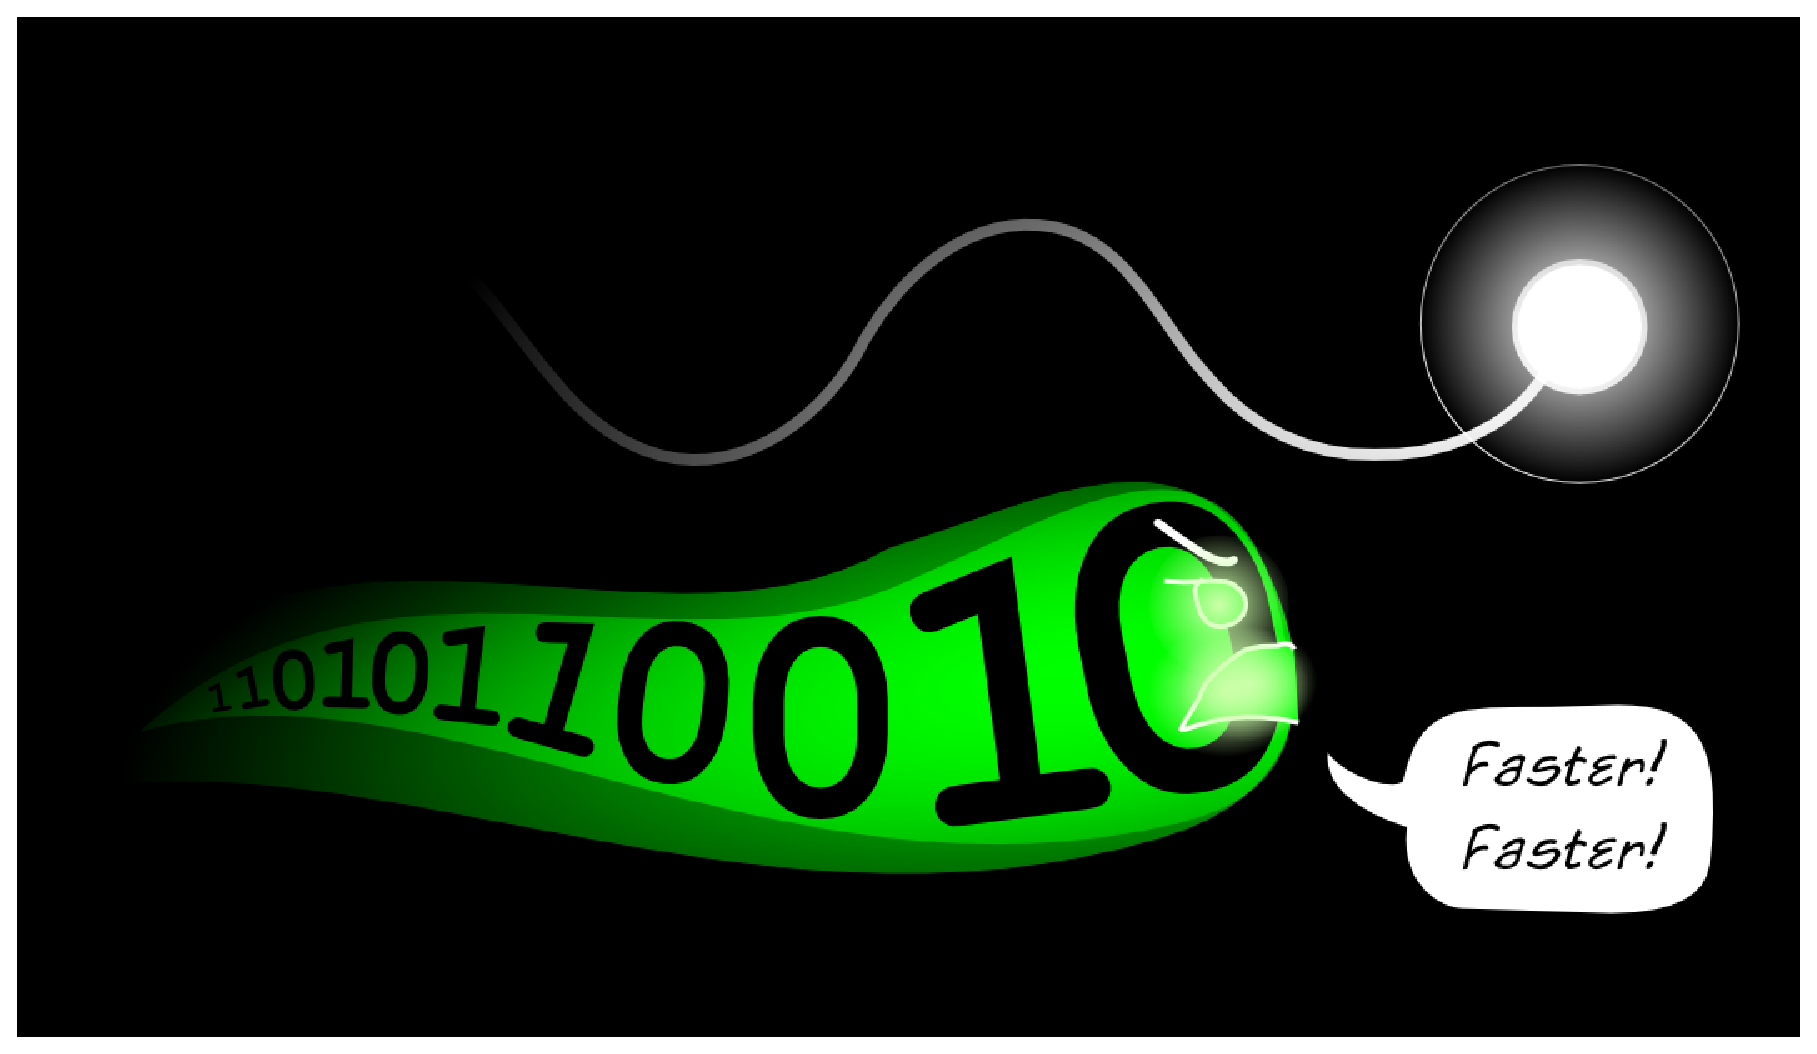
\includegraphics{cartoons/Data-chasing-light-wave}}
\caption{Hardware and Software: On Same Side}
\ContributedBy{Figure}{fig:cpu:Hardware and Software: On Same Side}{Melissa Broussard}
\end{figure}

In short, hardware and software engineers are really on the same side,
with both trying to make computers go fast despite the best efforts of
the laws of physics, as fancifully depicted in
Figure~\ref{fig:cpu:Hardware and Software: On Same Side}
where our data stream is trying its best to exceed the speed of light.
The next section discusses some additional things that the hardware engineers
might (or might not) be able to do, depending on how well recent
research translates to practice.
Software's contribution to this noble goal is outlined in the remaining
chapters of this book.
